
\documentclass[a4paper,12pt]{article} % тип документа


% Русский язык
\usepackage[T2A]{fontenc} % кодировка
\usepackage[utf8]{inputenc} % кодировка исходного текста
\usepackage[english,russian]{babel} % локализация и переносы


% Математика
\usepackage{amsmath,amsfonts,amssymb,amsthm,mathtools}


\usepackage{wasysym}

%Заговолок
\author{Талашкевич Даниил Александрович}

\title{Неделя 8. Комбинаторика II.
Биномиальные коэффициенты}

\date{\today}

\begin{document}

\maketitle
\thispagestyle{empty}

\newpage
\setcounter{page}{1}
\begin{center}
\itshape
\bfseries
{ \Large Problems:}
\end{center}

{\bf 1.} Робот ходит по координатной плоскости. На каждом шаге он может
увеличить одну координату на 1 или обе координаты на 2. Сколько
есть способов переместить Робота из точки (0, 0) в точку (4, 5)?
\begin{center}
\bfseries
{\Large Решение: }
\end{center}

В какую-либо точку с координатами $x,y \geqslant 2$ можно попасть $P(x,y) = P(x-1,y) + P(x,y-1) + P(x-2,y-2)$ способами, где $ \forall x,y \in \mathbb {N} \mapsto P(0,y) = P(x,0) = 1 $. В итоге получим, что $P(4,5) = 189$. Наглядно это видно на следующей картинке:

\begin{center}
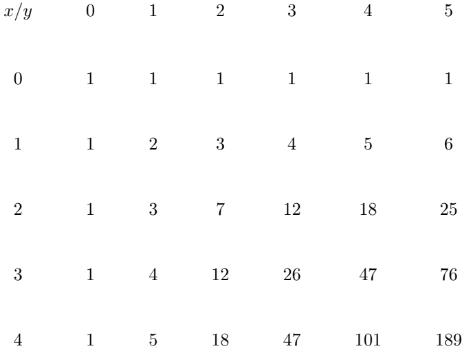
\includegraphics[scale = 0.8]{8 1}
\end{center}

\begin{flushright}
\begin{large}
\textbf {Ответ: $189$}
\end{large}
\end{flushright}

{\bf 2.} В магазине продается 10 видов пирожных. Сколькими способами
можно купить 100 пирожных (порядок покупки не важен)?
\begin{center}
\bfseries
{\Large Решение: }
\end{center}

Сопоставим вид пирожного со слагаемым $x_1$. У нас есть $10$ видов пирожных, значит у нас есть $10$ сопоставленных им слагаемым $X_i$ $(1 \leqslant i \leqslant 10)$.

Значение слагаемого $x_i$ означает количество выбранных пирожных этого вида $i$. Значит получаем следуюущю эквивалентную задачу, учитывая, что нужно выбрать $100$ пирожных: найти количество решений уравнения в целых неотрицательных числах:
\[x_1 + x_2 + ... + x_{10} = 100\]

Эта задача -- задача Муавра и имеет следующий ответ: количество решений равно $C^9_{109}$. Значит и исходная задача имеет такой же ответ

\begin{flushright}
\begin{large}
\textbf {Ответ:  $C^9_{109}$}
\end{large}
\end{flushright}

{\bf 3.} Какое слагаемое в разложении $(1 + 2)^n$ по формуле бинома Ньютона
будет наибольшим?
\begin{center}
\bfseries
{\Large Решение: }
\end{center}

$(a+b)^n = C_n^0\cdot a^n + C_n^1\cdot a^{n-1}b^1 + \cdots + C^n_n\cdot b^n$	. В данной задаче $a = 1$, тогда $(1+2)^n = C_n^0\cdot 1 + C_n^1\cdot 2^1 + \cdots + C^n_n\cdot 2^n$. Рассмотрим $k-$ый и $k+1-$ член в разложении по формуле бинома Ньютона: $\frac{x_k}{x_{k+1}} < 1$ -- условие, чтобы член разложения возрастал. Тогда $\frac{2^k n! (k+1)! (n-k-1)!}{2^{k+1} (n-k)! n!} < 1 \Rightarrow k < \frac{2n-1}{3}$.

Для $n = 0$ наибольший член -- первый.

Для $n = 1$ наибольший член -- второй.

Для всех остальных $n \geqslant 2$ имеем, что наибольший член под номером $\left[ \frac{2n-1}{3} \right] + 1$.


\begin{flushright}
\begin{large}
\textbf {Ответ: для $n \geqslant 2$ номер равен $\left[ \frac{2n-1}{3} \right] + 1$, частные случаи описаны в решении.}
\end{large}
\end{flushright}

{\bf 4.} Найдите число слов длины $n$ над алфавитом $\{0, 1\}$, в которых нет
двух единиц подряд.
\begin{center}
\bfseries
{\Large Решение: }
\end{center}

Рассмотрим последнюю цифру слова. Если она равна $1$, то предпоследняя цифра равна $0$ и нам нужно посчитать количество слов длины $n-2$. Если же она равна $0$, то ограничений на предпоследнее число нет, значит нужно найти количество слов длины $n-1$. Значит количество слов длины $n$ без двух единиц подряд $K(n)$ равно $K(n-1) + K(n-2)$.

Получили рекуррентную формулу, значит нужно задать начальные условия: у нас есть только $1$ слово без цифр и $2$ слова, состоящих из одной цифры. Значит получаем следующее: $K(n) = K(n-1) + K(n-2)$, $K(0) = 1, K(1) = 2$. очевидно, что $K(n) = F_{n+2}$, где $F_n$ -- $n$-ое число Фибоначии.


\begin{flushright}
\begin{large}
\textbf {Ответ: $F_{n+2}$ слов без двух единиц подряд}
\end{large}
\end{flushright}

{\bf 5.} Дать комбинаторное доказательство тождества

{\bf a) }${{n \choose m}} {{m \choose k}} = {{n \choose k}}{{ n - k \choose m - k }}$.  

{\bf б) }${{n \choose m}} = {{n - 2 \choose m}} +2{{n - 2 \choose m - 1}} {{n - 2 \choose m - 2}}$.
\newpage
\begin{center}
\bfseries
{\Large Решение: }
\end{center}

{\bf а)} Так как выбрать $m$ элементов из $n$ элементов тоже самое, что выбрать $n-m$ элементов из $n$ элементов, потому что если мы выберем $n-m$,то оставшиеся $m$ элементов будут однозначно определены и наоборот. Тогда $C^m_n = C^{n - m}_n$. Распишем что означает левая часть в исходном равенстве: сначала мы выбираем $m$ элементов из $n$ элементом, а потом из этих $m$ выбираем $k$ элементов. Это тоже самое, как показано выше, что и выбрать сначала $n-m$ элементов,а потом из оставшихся $k$ элементов.

Правая часть равенства: количество способов из $n$ выбрать $k$ элементов, а из оставшихся выбрать $m - k$. Это то же самое, что $C^k_n\cdot C^{n-m}_{n-k}$, опираясь на док-во в первой части решения.

Тогда имеем, что в первом случае мы сначала выбрали $n-m$ элементов, а потом $k$ из оставшихся, а во втором сначала выбрали $k$ элементов, а из оставшихся $n-m$, что одно и тоже.


{\bf б)} Воспользуемся тождеством Вандермонда: \[ {{m+n \choose r}=\sum _{k=0}^{r}{m \choose k}{n \choose r-k}}.\]

Докажем его: Предположим, что комитет состоит из $m$ мужчин и $n$ женщин. Сколькими способами можно сформировать подкомитет из $r$ членов? Ответом является

\[{ {m+n \choose r}.}\]
Это число является суммой по всем возможным значениям $k$ числа комитетов, состоящим из $k$ мужчин и $r-k$ женщин: \[ {\sum _{k=0}^{r}{m \choose k}{n \choose r-k}.}\]

Отсюда следует и доказательство исходного равенства.
	
	
\begin{flushright}
\begin{large}
\textbf {Ответ: доказано.}
\end{large}
\end{flushright}

{\bf 6.} Какое из чисел больше ${{F_{1000} \choose F_{998} + 1}}$ или ${{F_{1000} \choose F_{999} + 1}}$.
\begin{center}
\bfseries
{\Large Решение: }
\end{center}

Нам нужно сравнить два числа $C_{F_{1000}}^{F_{998} + 1}$ и $C_{F_{1000}}^{F_{999} + 1}$. Раскроем эти числа по определению:
\[\frac{1000!}{(F_{998} + 1)!(F_{1000} - F_{998} - 1)!} \text{ или } \frac{1000!}{(F_{999} + 1)!(F_{1000} - F_{999} - 1)!}\]
\[(F_{999} + 1)!(F_{1000} - F_{999} - 1)! \text{ или } (F_{998} + 1)!(F_{1000} - F_{998} - 1)!\]
\[(F_{999} + 1)!(F_{998} - 1)! \text{ или } (F_{998} + 1)!(F_{999} - 1)!\]
\[\frac{(F_{999} + 1)!(F_{998} + 1)!}{F_{998}(F_{998} + 1)} \text{ или } \frac{(F_{999} + 1)!(F_{998} + 1)!}{F_{999}(F_{999} + 1)}\]
\[F_{999}(F_{999} + 1) \text{ или } F_{998}(F_{998} + 1)\]
\[F_{999}(F_{999} + 1) > F_{998}(F_{998} + 1)\]

Значит изначальное число слева было больше.


\begin{flushright}
\begin{large}
\textbf {Ответ: $C_{F_{1000}}^{F_{998} + 1} > C_{F_{1000}}^{F_{999} + 1}$}
\end{large}
\end{flushright}

{\bf 7.} Приведите комбинаторное доказательство равенства \[ \sum\limits_{k = 0}^{(n+1)/2} {{n-k+1 \choose k}} = F_{n+2} .\]
\begin{center}
\bfseries
{\Large Решение: }
\end{center}

Рассмотрим множество последовательностей длины $n$, состоящих из $0$ и $1$, в которых не бывает двух $1$ стоящих рядом. Докажем, что количество таких последовательностей равно $F_{n + 2}$ (придадим числам Фибоначчи
комбинаторный смысл): 

Предположим, что имеется лента, разбитая на клетки и уходящая вправо до бесконечности. На первой клетке этой ленты сидит кузнечик. Из любой клетки кузнечик может перепрыгнуть либо на одну, либо на две клетки вправо. Тогда $a_n$ -- кол-во  способов, которыми кузнечик может добраться до $n$-ой клетки. Тогда $a_1 = a_2 = 1$. Кроме того, в $n + 1$-ую клетку кузнечик может попасть либо из $n$-ой клетки, либо перепрыгнув $n$-ую клетку. Поэтому $a_{n + 1} = a_{n - 1} + a_n$. Отсюда $a_n = F_{n - 1} \Rightarrow F_{n+2} = F_{n + 1} + F_{n}$. Тогда, если каждую клетку обозначит за 1 или 0 в соответствии с тем, как прыгай заяй от этой клетки: 1 -- если через 1 клетку  и 0 если на следующюю соответственно получаем, что 2 стоящие рядом единицы не могут быть, потому что если в одной стоит единица, то на следующей клетке заяц не мог оказаться и, соответсвенно, там не может стоять единица.

Теперь, когда мы придали числам Фибоначчи комбинаторный смысл докажем равенство:

Число единиц в последовательности обозначим через $k$. Ясно, что  $0\leqslant k\leqslant\frac{n+1}{2}.$ При фиксированном $k\geqslant1$ поступаем так: для всех единиц, кроме последней, следующее число равно нулю. Вычеркнем эти нули в количестве $k-1$ штуки. Останется $n-k+1$ член, среди которых $k$ единиц. Таких последовательностей $C^k_{n-k+1}$. Для каждой из них можно однозначно вернуться назад, вписав нули после каждой из единиц кроме самой последней. При $k=0$ эта же формула также даёт верный результат, равный единице. Остаётся просуммировать сочетания по всем возможным $k$ таким, что $0\leqslant k\leqslant\frac{n+1}{2}$, что дает такое результат: \[  \sum\limits_{k = 0}^{(n+1)/2} {{n-k+1 \choose k}} = F_{n+2} .\]


\begin{flushright}
\begin{large}
\textbf {Ответ: доказано}
\end{large}
\end{flushright}

{\bf 8.} Сколько способов разместить 20 различных книг на 5 полках, если
каждая полка может вместить все 20 книг? Размещения, отличающиеся
порядком книг на полках, считаются различными.
\begin{center}
\bfseries
{\Large Решение: }
\end{center}

Задачу можно свести к такой: у нас есть $20$ книг и $4$ разделителя и нам нужно по порядку расставить книги и разделители и посчитать количество таких расстановок. Ограничений на то, что разделители не могут находится рядом, нет, так как в полке могут и не находится книги.

Так как нам важен порядок книг, но все разделители считаются одинаковыми, то нам нужно посчитать количество перестановок $24$ объектов с учётом того, что нам не важен порядок разделителей, так как они все эквивалентны. Отсюда получаем $\frac{24!}{4!}$ способов, где $4!$ и есть поправка на разделители.

\begin{flushright}
\begin{large}
\textbf {Ответ: $\frac{24!}{4!}$ способа}
\end{large}
\end{flushright}

{\bf 9.} Студсовет из 8 человек выбирает из своего состава председателя
путем тайного голосования. Каждый может отдать один голос за любого
члена студсовета. Результат голосования – число голосов, отданных
за каждого кандидата. Сколько существует различных результатов
голосования?
\newpage
\begin{center}
\bfseries
{\Large Решение: }
\end{center}

Представим, что у нас есть $8$ единиц и нам нужно выбрать $7$ мест, куда поставить палочки между ними, таким образом разграничим их на $8$ целых слагаемых, не меньше нуля. Выбрать $7$ позиций палочек можно следующим образом: добавим $7$ позиций, тогда нужно расставить $7$ палочек среди $7+8$ позиций, тогда итоговый ответ $C^7_{15}$.

\begin{flushright}
\begin{large}
\textbf {Ответ: $C^7_{15}$}
\end{large}
\end{flushright}

{\bf 10.} Сколькими способами можно переставить буквы в слове «ОБОРО-
НОСПОСОБНОСТЬ», так чтобы две буквы «О» не стояли рядом?
\begin{center}
\bfseries
{\Large Решение: }
\end{center}

В слове "ОБОРОНОСПОСОБНОСТЬ"\ всего $18$ букв, $7$ из которых -- буква "О".

Рассмотрим для начала слово без букв "О". Количество перестановок равно
\[k = \frac{11!}{2!2!3!}\]

Далее включим в это слово все буквы. Наша цель -- расставить их между буквами слова таким образом, чтобы у нас не стояли две буквы "О"\ подряд, то есть нельзя ставить больше одной буквы между словами. У нас есть $11$ букв в слове, то есть $12$ мест, куда можно вставить буквы "О". Из этих $12$ мест нам нужно выбрать $7$ -- $C^7_{12}$ способов.

Итого получим $kC^7_{12} = \frac{11!12!}{2!2!3!5!7!}$ способов.

\begin{flushright}
\begin{large}
\textbf {Ответ:  $\frac{11!12!}{2!2!3!5!7!}$ способов}
\end{large}
\end{flushright}


{\bf 11.} Вы купили в магазине набор из 30 бусинок. Бусинки бывают 15 разных цветов, каждого цвета по две штуки. Сколькими способами можно составить, используя все бусинки, круглое ожерелье, если ожерелья, которые совмещаются вращением в пространстве, считать
одинаковыми. Более формально, два ожерелья одинаковые, если одно
можно совместить с другим так, чтобы они совпали.
\newpage
\begin{center}
\bfseries
{\Large Решение: }
\end{center}

Для начала разорвём ожерелье в некотором месте, представив его в виде линии из $30$ бусинок. Найдём количество всех возможных комбинаций рамещения бусинок, учитывая, что есть по $2$ бусинки $15$ различных цветов. Очевидно, что количество таких размещений равно
\[S_0 = \frac{30!}{(P_2)^{15}} = \frac{30!}{(2!)^{15}}\]

Теперь соберём начало и конец лнии вместе -- получим ожерелье. Теперь нам нужно учесть, что мы посчитали некоторые одинаковые комбинации более одного раза, так как мы не учитывали поворот ожерелья в пространстве. Учтём, что мы посчитали одну и ту же комбинацию $30$ раз, так как можно получить $30$ сдвигов в линии из $30$ бусинок.

Теперь учтём, что можно зеркально отразить некоторое ожерелье, получив другое или то же самое ожерелье. Мы получим другое ожерелье только в том случае, если исходное ожерелье хирально.

Найдём количество нехиральных комбинаций. Рассмотрим две произвольные бусинки одинакового цвета. Пусть кратчайшее расстояние между ними $k$ бусинок, то есть на этом расстоянии между двумя бусинками находятся $k-1$ других бусинок, причём их цвет отличается от выбранных ранее двух бусинок. При отзеркаливании рассматриваемой комбинации нумерация этих $k-1$ бусинок меняется на обратную, так как направление по часовой стрелке изменилось на направление против часовой, но по обоим направлениям должны быть одни и те же бусинки. Отсюда сразу следует, что $k-1$ -- чётное число и нехиральная комбинация имеет следующий вид: берём случайную комбинацию из $15$ бусинок различных цветов, дублируем эту комбинацию, а затем соединяем концы и начала эти одинаковых комбинаций. Очевидно, что при отражении такой комбинации в зеркале получается та же самая комбинация.

Теперь подсчитаем количество таких нехиральных комбинаций: у нас есть $15!$ способов собрать комбинацию из $15!$ бусинок различного цвета. Значит и количество нехиральных комбинаций равно $15!$.

С учётом всего ранее написанного имеем следующее количество комбинаций бусинок в ожерелье:
\[S_1 = \frac{15!}{2} + \frac{S_0}{30} - 15! = \frac{29!}{2^{15}} - \frac{15!}{2}\]

\begin{flushright}
\begin{large}
\textbf {Ответ: $\frac{29!}{2^{15}} - \frac{15!}{2}$ способов}
\end{large}
\end{flushright}


\end{document}
